\subsection{Data Lifecycle}

\indent 

The Data Lifecycle is a fundamental concept in information security and 
data governance. It shows how data is created, used, stored, and eventually disposed of. Understanding this is critical for IT professionals because security controls must be applied at every stage. Data doesn’t stay static - it passes through stages. A common model has 6–7 stages (some frameworks differ slightly).

\begin{figure}[h!]
    \centering
    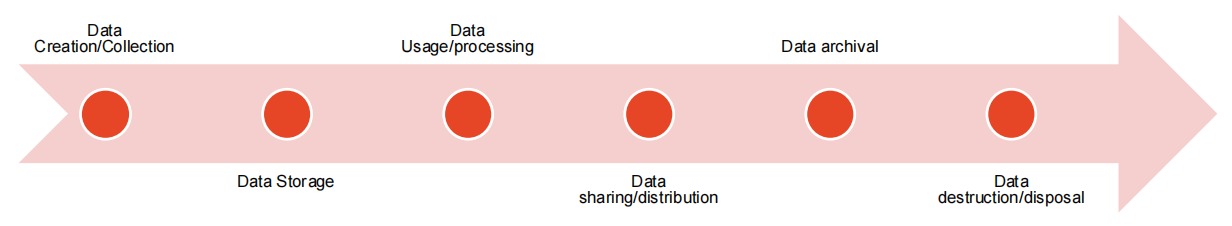
\includegraphics[width=0.9\linewidth]{figures/Week 10/Typical Data Lifecycle.png}
    \caption{A typical Data Lifecycle}
\end{figure}

\bigskip

\noindent\textbf{Data Creation/Collection}

Data is generated or collected from users, devices, or systems.

Examples: User registration forms, IoT sensors, employee records.

Security focus: Collect only necessary data (minimization). Secure input validation. Ensure informed consent at the point of collection.

\bigskip

\noindent \textbf{Data Storage}

Data is stored in databases, data warehouses, or cloud storage.

Security focus: Encryption at rest. Access controls (who can read/write). Redundancy and backups to prevent loss.

\bigskip

\noindent\textbf{Data Usage/Processing}

Data is used for operations, analytics, or decision-making.

Examples: HR system retrieving employee details, algorithms analyzing customer behavior.

Security focus: Encryption in use (confidential computing). Role-based access control. Audit logs of who accessed/modified data.

\bigskip

\noindent\textbf{Data Sharing/Distribution}

Data is shared internally (between departments) or externally (with partners, vendors, regulators).

Security focus: Encryption in transit (TLS/SSL, VPN). Data masking/anonymization for third parties. Contracts/agreements ensuring compliance with privacy laws.

\bigskip

\noindent\textbf{Data archival}

Data that’s no longer actively used but must be retained for compliance, historical, or business reasons.

Examples: Old financial records, patient health records.

Security focus: Secure long-term storage. Retrieval controls (only authorized users). Legal retention schedules (e.g., tax records for 7 years).

\noindent\textbf{Data Destruction/Disposal}

Data that’s no longer needed is securely destroyed.

Security focus: Shredding physical documents. Wiping/overwriting disks (DoD 5220.22-M, NIST standards). Cryptographic erasure in cloud environments.

\subsubsection{Security across the lifecycle}

\indent

At every stage, IT professionals must apply:

\begin{itemize}
    \item Confidentiality: Limit access to only those who need it.
    \item Integrity: Ensure data is accurate and not tampered with.
    \item Availability: Ensure authorized users can access data when required.
\end{itemize}

Data breaches often occur because organizations forget to protect “inactive” or “archived” data.

Regulations like GDPR require organizations to know where data is in its lifecycle.

Secure lifecycle management prevents unauthorized access, misuse, and legal non-compliance.

\subsection{Governance Frameworks}

\subsubsection{Governance Frameworks for Information Security}

\indent

\textbf{Information security governance} is about \textbf{establishing policies, procedures, and controls} so that information assets are protected and aligned with business objectives. 

Several widely-recognized frameworks help IT professionals do this.

A few examples of such frameworks are:

\begin{itemize}
    \item ITIL (Information Technology Infrastructure Library) - Covered in W6
    \item COBIT (Control Objectives for Information and related Technologies ) - W6
    \item NIST (National Institute of Standards and Technology)
    \item GDPR (General Data Protection Regulation)
\end{itemize}

\subsubsection{NIST Cybersecurity Framework (CSF)}

\indent

Origin: Developed by the National Institute of Standards and Technology (NIST), USA, primarily for critical infrastructure but widely adopted globally.

The main purpose of this framework was to:

\begin{itemize}
    \item Provide a risk-based approach to manage and improve cybersecurity.
    \item Be flexible enough to be adapted by organizations of all sizes and sectors.
\end{itemize}

Key benefits of NIST CSF:

\begin{itemize}
    \item Provides common language for cybersecurity discussions.
    \item Helps prioritize security investments based on risk exposure.
    \item Encourages continuous improvement.
\end{itemize}

The core components of NIST CSF are:

\begin{itemize}
    \item Framework Core (5 functions)
        \begin{itemize}
            \item Identify: Understand organizational assets, systems, data, and risks.
            \item Protect: Implement safeguards to limit or contain impact of cyber incidents.
            \item Detect: Identify cybersecurity events promptly.
            \item Respond: Act quickly to incidents to mitigate impact.
            \item Recover: Restore services and capabilities after an incident
        \end{itemize}
    \item Implementation Tiers
        \begin{itemize}
            \item Tier 1 (Partial): Cybersecurity is ad hoc and reactive, with informal or inconsistent practices.
            \item Tier 2 (Risk-informed): Cybersecurity policies exist but are applied inconsistently, with partial risk awareness.
            \item Tier 3 (Repeatable): Cybersecurity practices are formally documented, consistently applied, and monitored.
            \item Tier 4 (Adaptive): Cybersecurity is fully integrated, continuously improved, and adapts to evolving threats.
        \end{itemize}
    \item Profiles: Customized alignment of framework functions and categories with the organization’s business needs and risk tolerance.
\end{itemize}

\subsubsection{GDPR}

\indent 

Origin: European Union regulation, effective May 2018.

The main purpose for this regulation was to:

\begin{itemize}
    \item Protect the personal data and privacy rights of EU citizens.
    \item Standardize data protection laws across EU countries.
    \item Give individuals more control over their data.
\end{itemize}

Under this regulation, individuals have the following rights:

\begin{itemize}
    \item Right to access, rectify, erase, restrict processing, data portability, and object (covered in your “Individual Rights of Data” section).
    \item Right not to be subject to automated decision-making that significantly affects them.
\end{itemize}

Key principles of GDPR:

\begin{itemize}
    \item Lawfulness, Fairness, and Transparency: Data must be processed legally, fairly, and transparently.
    \item Purpose Limitation: Data collected for specific purposes only.
    \item Data Minimization: Collect only what’s necessary.
    \item Accuracy: Keep data accurate and up to date.
    \item Storage Limitation: Retain data only as long as necessary.
    \item Integrity and Confidentiality: Protect data against unauthorized access, loss, or damage.
    \item Accountability: Organizations must demonstrate compliance
\end{itemize}

\subsection{Cybersecurity Standards and Best practices}

\subsubsection{Cybersecurity}

\indent 

\textbf{Cybersecurity} is the practice of \textbf{protecting computers, networks, programs, and data from unauthorized access, attacks, damage, or theft.} It focuses specifically on the \textbf{digital aspect} of information security.

Cybersecurity is often aligned with the CIA Triad:

\begin{itemize}
    \item Confidentiality: Ensure that sensitive information is accessed only by authorized users.
    \item Integrity: Protect data from being altered or tampered with.
    \item Availability: Ensure systems and data are accessible to authorized users when needed.
\end{itemize}

\subsubsection{Domains of Cybersecurity}

\begin{itemize}
    \item \textbf{Network Security}: Protecting networks and connected devices from breaches and attacks.
    \item \textbf{Application Security}: Ensuring software is free of vulnerabilities and secure from threats.
    \item \textbf{Information Securit}y: Protecting data both at rest and in transit.
    \item \textbf{Operational Security (OPSEC)}: Policies and procedures to protect organizational processes.
    \item \textbf{Endpoint Security}: Protecting devices like computers, smartphones, and IoT devices.
    \item \textbf{Cloud Security}: Securing cloud-based infrastructure, applications, and data.
    \item \textbf{Identity \& Access Management (IAM)}: Controlling who can access what resources
\end{itemize}

\subsubsection{Common Cybersecurity Practices}

\begin{itemize}
    \item Use \textbf{strong passwords} and \textbf{multi-factor authentication (MFA)}.
    \item Keep software and systems \textbf{updated and patched}.
    \item Implement \textbf{firewalls, VPNs, and intrusion detection systems}.
    \item \textbf{Encrypt data} in transit and at rest.
    \item Train staff on \textbf{phishing, social engineering, and safe online behavior}.
    \item Develop an \textbf{incident response plan} for security breaches.
    \item Regularly \textbf{monitor systems and audit logs} for suspicious activity.
\end{itemize}

\subsubsection{Cybersecurity Standards}

\indent 

Cybersecurity standards provide organizations with structured guidelines, best practices, and controls to protect their digital assets. They help ensure consistency, compliance, and risk management across industries.

A few common cybersecurity standards are:

\begin{itemize}
    \item ISO/IEC 27001
    \item NIST Cybersecurity Framework
    \item PCI DSS (Payment Card Industry Data Security Standard)
    \item HIPAA Security Rule (Healthcare)
\end{itemize}

\subsubsection{PCI DSS – Payment Card Industry Data Security Standard}

\indent

The main purpose is to: Protect payment card data and reduce the risk of fraud for organizations that store, process, or transmit credit/debit card information. Developed by the PCI Security Standards Council (founded by Visa, MasterCard, Amex, Discover, and JCB).

The scope of this standard: Applies to any organization involved in payment card transactions, including merchants, processors, and service providers.

Key requirements of PCI DSS:

\begin{itemize}
    \item \textbf{Build and maintain a secure network}: Install and maintain a firewall to protect cardholder data. Do not use vendor-supplied default passwords.
    \item \textbf{Protect cardholder data}: Encrypt data in storage and in transit.
    \item \textbf{Maintain a vulnerability management program}: Use anti-virus and regularly update software.
    \item \textbf{Implement strong access control measures}: Restrict access to cardholder data by need-to-know. Assign unique IDs to users.
    \item \textbf{Monitor and test networks regularly}: Track and monitor all access to network resources and cardholder data. Regularly test security systems.
    \item \textbf{Maintain an information security policy}: Establish policies for employees and contractors.
\end{itemize}

\subsubsection{HIPAA – Health Insurance Portability and Accountability Act}

\indent 

The main purpose of this act is to: Protect \textbf{electronic protected health information (ePHI)} in the \textbf{healthcare industry}. Ensures confidentiality, integrity, and availability of patient health data.

The scope of this act: Applies to covered entities (healthcare providers, health plans, clearinghouses) and business associates (service providers handling ePHI).

Consequences of non-compliance: Civil penalties: \$100–\$50,000 per violation, up to \$1.5 million annually. Criminal penalties for knowingly violating HIPAA. Loss of reputation and patient trust.

HIPAA Security Rule Safeguards:

\begin{itemize}
    \item Administrative Safeguards
        \begin{itemize}
            \item Security management processes (risk analysis and mitigation).
            \item Workforce training on privacy and security policies.
            \item Contingency planning and incident response.
        \end{itemize}
    \item Physical Safeguards
        \begin{itemize}
            \item Facility access controls.
            \item Secure storage for servers, workstations, and paper records.
            \item Policies for device and media handling.
        \end{itemize}
    \item Technical Safeguards
        \begin{itemize}
            \item Access controls (unique IDs, passwords, and role-based access).
            \item Audit controls (tracking system activity).
            \item Integrity controls (ensure data is not improperly altered).
            \item Encryption of ePHI in storage and transmission.
        \end{itemize}
\end{itemize}

\subsection{Threat Modeling and Incident Response}

\subsubsection{Threat Modelling}

\indent 

Threat modelling is a \textbf{structured approach to identifying, understanding, and prioritizing potential security threats} to a system, application, or organization. It helps \textbf{anticipate attacks before they happen}.

The main purpose of threat modelling is to:

\begin{itemize}
    \item Identify \textbf{vulnerabilities} in systems or processes.
    \item Prioritize security measures based on \textbf{risk and potential impact}.
    \item Improve \textbf{design and architecture} with security in mind.
\end{itemize}

\subsubsection{STRIDE – Threat Modelling framework}

\indent 

STRIDE is a systematic framework for identifying security threats in software systems, applications, and IT infrastructure. It stands for 6 types of threats:

\begin{itemize}
    \item Spoofing Identity (S): When an attacker \textbf{pretends to be someone else} to gain unauthorized access.
    \item Tampering with Data (T): Unauthorized \textbf{modification of data} in storage, transit, or during processing.
    \item Repudiation (R): When a user \textbf{denies performing an action}, and the system lacks proof to dispute it.
    \item Information Disclosure (I): Unauthorized \textbf{exposure of sensitive information}.
    \item Denial of Service (D): Attacks that \textbf{make a system or service unavailable} to legitimate users.
    \item Elevation of Privilege (E): When a user or process \textbf{gains higher privileges} than intended
\end{itemize}

\subsubsection{Mitigation Strategies for STRID}

\begin{table}[h!]
\centering
\begin{tabular}{cl}
\hline
\textbf{Threat}                     & \multicolumn{1}{c}{\textbf{Mitigation Strategies}}                                                                                                              \\ \hline
\textbf{Spoofing Identity (S)}      & \begin{tabular}[c]{@{}l@{}}Multi-factor authentication (MFA)\\ Strong identity verification\\ Secure token-based authentication\end{tabular}                    \\
\textbf{Tampering with Data (T)}    & \begin{tabular}[c]{@{}l@{}}Digital signatures and checksums\\ Encryption of data in transit and at rest\\ Access controls with audit logs\end{tabular}          \\
\textbf{Repudiation (R)}            & \begin{tabular}[c]{@{}l@{}}Logging and audit trails\\ Non-repudiation mechanisms like digital signatures\\ Immutable storage for critical logs\end{tabular}     \\
\textbf{Information Disclosure (I)} & \begin{tabular}[c]{@{}l@{}}Encryption of sensitive data\\ Data classification and masking\\ Strong access controls and network segmentation\end{tabular}        \\
\textbf{Denial of Service (D)}      & \begin{tabular}[c]{@{}l@{}}Rate limiting and throttling\\ Load balancing and redundancy\\ Monitoring and automated alerting\end{tabular}                        \\
\textbf{Elevation of Privilege (E)} & \begin{tabular}[c]{@{}l@{}}Principle of least privilege (PoLP)\\ Regular patching and vulnerability management\\ Role-based access controls (RBAC)\end{tabular} \\ \hline
\end{tabular}
\end{table}

\subsubsection{Incident Response Plan}

\indent 

An \textbf{Incident Response Plan} is a \textbf{structured approach for detecting, responding to, and recovering from cybersecurity incidents}. It ensures that organizations \textbf{minimize damage, restore operations quickly, and meet legal and regulatory obligations}.

The main goal of an IRP is to:

\begin{itemize}
    \item Reduce \textbf{impact of cyber incidents} (financial, operational, reputational).
    \item Ensure \textbf{business continuity}.
    \item Learn from incidents to \textbf{improve future security posture}.
\end{itemize}

\subsubsection{Incident Response Lifecycle}

\indent 

\begin{itemize}
    \item Preparation
        \begin{itemize}
            \item Establish \textbf{policies, procedures, and tools} before an incident occurs.
            \item Train staff and \textbf{create an Incident Response Team (IRT)}.
            \item Implement monitoring and logging systems.
        \end{itemize}
    \item Identification
        \begin{itemize}
            \item Detect potential incidents \textbf{as early as possible}.
            \item Determine \textbf{scope, type, and severity} of the incident.
        \end{itemize}
    \item Containment
        \begin{itemize}
            \item \textbf{Limit the spread and impact} of the incident.
            \item \textbf{Short-term containment}: Immediate action to prevent further damage.
            \item \textbf{Long-term containment}: Implement fixes while maintaining operations
        \end{itemize}
    \item Eradication: \textbf{Remove the root cause} of the incident from the environment.
    \item Recovery
        \begin{itemize}
            \item \textbf{Restore affected systems and services} to normal operations.
            \item Ensure that systems are \textbf{fully functional, secure, and verified}.
            \item Monitor systems for \textbf{residual threats or recurring issues}.
        \end{itemize}
    \item Lessons Learned
        \begin{itemize}
            \item Conduct a \textbf{post-incident review}.
            \item Identify what went well? What could be improved? Gaps in policies or tech
            \item Update the \textbf{IRP, security controls, and employee training}.
            \item Document findings for \textbf{regulatory and audit purposes}.
        \end{itemize}
\end{itemize}

\subsubsection{Disaster Recovery Plan}

\indent 

A \textbf{Disaster Recovery Plan (DRP)} is a documented, structured approach that outlines \textbf{how an organization will recover IT systems, data, and operations after a disruptive event}, such as a cyberattack, hardware failure, natural disaster, or human error.

The goal is to:

\begin{itemize}
    \item \textbf{Minimize downtime} and data loss.
    \item \textbf{Ensure business continuity}.
    \item Protect critical systems and resources.
    \item Meet \textbf{regulatory and contractual requirements}.
\end{itemize}

\subsubsection{Disaster Recovery Strategies}

\begin{itemize}
    \item \textbf{Cold Site}: Pre-prepared physical location with basic infrastructure; requires setup during disaster.
    \item \textbf{Warm Site}: Partially equipped backup site; servers and data need configuration before use.
    \item \textbf{Hot Site}: Fully operational duplicate environment; can take over immediately during disaster.
    \item \textbf{Cloud-Based DR / DRaaS (Disaster Recovery as a Service)}: Replicate systems/data to cloud for rapid recovery.
    \item \textbf{Backup and Restore}: Regular backups stored offsite; slower recovery but cost-effective.
\end{itemize}

\bigskip

\noindent\textbf{Difference between IRP and DRP}

\begin{table}[h!]
\centering
\renewcommand{\arraystretch}{1.35}
\begin{tabular}{|p{3cm}|p{6.2cm}|p{6.2cm}|}
\hline
\textbf{Feature} & \textbf{Disaster Recovery Plan (DRP)} & \textbf{Incident Response Plan (IRP)} \\
\hline

\textbf{Focus} & Restoring IT systems, data, and operations after a disaster &
Detecting, containing, and mitigating cybersecurity incidents \\
\hline

\textbf{Objective} & Minimize downtime and data loss &
Minimize damage and contain threats \\
\hline

\textbf{Scope} & IT infrastructure, applications, backups &
Security incidents, breaches, attacks \\
\hline

\textbf{Timing} & Post-disaster recovery &
During and immediately after an incident \\
\hline

\textbf{Best Practices} &
\begin{itemize}
    \item Test the plan at least annually, or after major infrastructure changes
    \item Use redundancy and failover mechanisms (servers, networks, power supply)
    \item Maintain clear documentation accessible to authorized personnel
    \item Ensure regulatory compliance for data protection and recovery
    \item Align DRP with Incident Response Plan (IRP) and Business Continuity Plan (BCP)
\end{itemize}
&
\begin{itemize}
    \item Keep the plan up-to-date with evolving threats
    \item Conduct regular drills and tabletop exercises
    \item Use automated monitoring and alerting for faster detection
    \item Apply the principle of least privilege in access control
    \item Maintain offsite backups and redundant systems
    \item Integrate threat intelligence to anticipate attacks
\end{itemize}
\\
\hline

\end{tabular}
\caption{Difference between Disaster Recovery Plan (DRP) and Incident Response Plan (IRP)}
\end{table}

\subsubsection{Business Continuity Plan}

\indent 

A \textbf{Business Continuity Plan} is a \textbf{proactive strategy and documented plan} that ensures an organization can \textbf{continue essential operations during and after a disruptive event}, whether it’s a cyberattack, natural disaster, equipment failure, or other crises.

The main goal is to:

\begin{itemize}
    \item Maintain \textbf{critical business functions} during disruptions.
    \item Minimize \textbf{financial, operational, and reputational impact}.
    \item Ensure \textbf{employee, customer, and stakeholder confidence}.
    \item Complement \textbf{Disaster Recovery (DRP)} for IT systems.
\end{itemize}

\subsubsection{BCP Lifecycle}

\begin{itemize}
    \item \textbf{Project Initiation and Management}: Establish objectives, scope, and resources.
    \item \textbf{Business Impact Analysis (BIA)}: Identify critical functions and prioritize recovery.
    \item \textbf{Risk Assessment}: Evaluate threats and vulnerabilities.
    \item \textbf{Strategy Development}: Define recovery strategies for critical processes.
    \item \textbf{Plan Development}: Document procedures, roles, and resources.
    \item \textbf{Testing and Exercises}: Conduct drills to validate the plan.
    \item \textbf{Maintenance and Continuous Improvement}: Update plan based on lessons learned and changes in business.
\end{itemize}

\subsubsection{Best practices for BCP}

\begin{itemize}
    \item Align BCP with \textbf{DRP and IRP} for a complete resilience strategy.
    \item Identify and protect \textbf{key resources}, including staff, technology, facilities, and suppliers.
    \item Ensure \textbf{communication plans} are tested and accessible.
    \item Perform \textbf{regular audits and plan updates}.
    \item Use \textbf{cloud services and remote capabilities} to increase flexibility.
    \item Involve \textbf{leadership support} for faster decision-making during crises.
\end{itemize}

\subsection{Modern IT Security}

\indent 

Modern threats are evolving rapidly and often target humans, technology, and processes simultaneously. Security is no longer just IT’s responsibility, it requires an organization-wide approach. Proactive, layered defense using policies, technology, awareness, and continuous monitoring is essential. Integration of cybersecurity frameworks and standards (like NIST, ISO 27001, PCI DSS, HIPAA) is critical for resilience.

\subsubsection{Modern IT Security Challenges}

\begin{itemize}
    \item Cloud adoption risks
        \begin{itemize}
            \item Challenge: Increased attack surface due to distributed workforce and BYOD (Bring Your Own Device).
            \item Key issues may include misconfigurations, shared responsibility confusion, API vulnerabilities, etc.
        \end{itemize}
    \item Remote work security challenges
        \begin{itemize}
            \item Challenge: Increased attack surface due to distributed workforce and BYOD (Bring Your Own Device).
            \item Key issues may include usage of unsecured home networks, lack of enterprise security controls on personal devices, etc.
        \end{itemize}
    \item Shadow IT Challenge: Employees using unauthorized applications or cloud services without IT oversight.
\end{itemize}

\subsubsection{Cloud Deployment Models}

\begin{table}[htbp]
\centering
\renewcommand{\arraystretch}{1.3}
\begin{tabular}{|p{3.2cm}|p{7cm}|p{4.5cm}|}
\hline
\textbf{Model} & \textbf{Description} & \textbf{Example} \\
\hline

\textbf{Public Cloud} &
Services offered over the internet by third-party providers; shared infrastructure &
AWS, Microsoft Azure, Google Cloud \\
\hline

\textbf{Private Cloud} &
Cloud infrastructure dedicated to a single organization; more control and security &
VMware vSphere, OpenStack \\
\hline

\textbf{Hybrid Cloud} &
Combines public and private clouds; flexible workload distribution &
On-premises + Azure/AWS integration \\
\hline

\textbf{Community Cloud} &
Shared infrastructure for a specific group or industry &
Government or healthcare consortia clouds \\
\hline

\end{tabular}
\caption{Cloud Deployment Models}
\end{table}

\subsubsection{Cloud Service Models}

\begin{table}[htbp]
\centering
\renewcommand{\arraystretch}{1.3}
\begin{tabular}{|p{4cm}|p{7.2cm}|p{4cm}|}
\hline
\textbf{Model} & \textbf{Description} & \textbf{Example} \\
\hline

\textbf{Infrastructure as a Service (IaaS)} &
Provides virtualized computing resources (servers, storage, network) &
AWS EC2, Google Compute Engine \\
\hline

\textbf{Platform as a Service (PaaS)} &
Provides platform for application development and deployment &
Google App Engine, Microsoft Azure App Service \\
\hline

\textbf{Software as a Service (SaaS)} &
Provides fully managed software accessible via web &
Microsoft 365, Salesforce, Zoom \\
\hline

\textbf{Function as a Service (FaaS) / Serverless} &
Runs code without managing servers; triggered by events &
AWS Lambda, Azure Functions \\
\hline

\end{tabular}
\caption{Cloud Service Models}
\end{table}

\subsubsection{Security for Cloud and Virtualised Environments}

\indent 

Cloud and virtualization introduce \textbf{flexibility and scalability}, but they also create \textbf{new security challenges}. Security must cover \textbf{infrastructure, platforms, applications, and data} across \textbf{public, private, and hybrid environments}.

A few emerging security technologies are:

\begin{itemize}
    \item \textbf{Zero Trust Architecture}: “Never trust, always verify” for cloud users and devices.
    \item \textbf{Container Security}: Protect Kubernetes and Docker environments.
    \item \textbf{Cloud Workload Protection Platforms (CWPP)}: Monitor VMs, containers, and serverless workloads.
    \item \textbf{AI-Driven Threat Detection}: Detect anomalous behavior in cloud traffic.
\end{itemize}

\subsubsection{Cloud environment security best practices}

\begin{itemize}
    \item \textbf{Secure the Hypervisor}: Only authorized personnel access; patch regularly.
    \item \textbf{Encrypt Data}: At rest, in transit, and during backup.
    \item \textbf{Strong Identity Management}: RBAC, MFA, SSO for cloud access.
    \item \textbf{Monitor Logs and Network Traffic}: Centralized logging, SIEM integration.
    \item \textbf{Micro-Segmentation}: Limit lateral movement in virtual networks.
    \item \textbf{Regular Vulnerability Assessments}: Scan VMs, containers, and cloud workloads.
    \item \textbf{Secure Configuration}: Follow vendor-recommended security baselines (CIS benchmarks).
    \item \textbf{Automated Security Tools}: Use Cloud Security Posture Management (CSPM) and container security solutions.
\end{itemize}

\subsection{Questions}

\subsubsection{End of Lecture Questions}

\begin{itemize}
    \item Describe the data life cycle and explain why each stage needs protection.
    \item What is the difference between NIST and GDPR frameworks in security management?
    \item List common cyber-security practices to protect an organization from threats.
    \item Explain the difference between incident response, disaster recovery, and business continuity plans.
    \item What are the main cloud deployment and service models, and how do they differ?
    \item Name at least three modern IT security challenges introduced by cloud adoption and remote work.
\end{itemize}

\subsubsection{Case Study}

\indent 

CloudSafe Corp is a mid-sized company providing SaaS solutions for healthcare providers. The company recently migrated 70\% of its applications to a hybrid cloud model while keeping sensitive patient records on a private cloud. Employees are working remotely, and collaboration occurs via Slack, Microsoft Teams, and cloud storage.

Incident: One morning, the IT team detects abnormal activity: a ransomware strain has encrypted several production servers in the public cloud. Several employees report being unable to access shared files. The attack appears to have entered via a phishing email targeting remote employees, exploiting weak MFA implementation. Some VMs hosting the SaaS application are offline, impacting service delivery.

Current Status:

\begin{itemize}
    \item Private cloud data is safe but some hybrid cloud services are down.
    \item Incident response is partially executed, but some teams are unclear on responsibilities.
    \item Customers have reported outages, and media attention is rising
\end{itemize}

\noindent\textbf{Case Study based Questions}:

\begin{itemize}
    \item Identify at least three security failures that contributed to the ransomware attack.
    \item Explain how the hybrid cloud deployment model influenced the impact of this incident.
    \item What incident response steps should CloudSafe Corp implement immediately to contain the ransomware?
    \item Suggest backup and disaster recovery strategies for minimizing downtime in this scenario.
    \item Discuss the role of identity and access management (IAM) in preventing similar attacks.
    \item Design a high-level incident response checklist for CloudSafe Corp during a ransomware outbreak.
\end{itemize}